\chapter{Wcześniejsze rozwiązania}\label{r:losers}
W chwili obecnej nie ma czegoś takiego jak język dostosowany do potrzeb sumerologów. Są strony internetowe oferujące wyszukiwanie za pomocą formularzy.
\section{The Cuneiform Digital Library Initiative}
\begin{figure}[h]
 \centering
 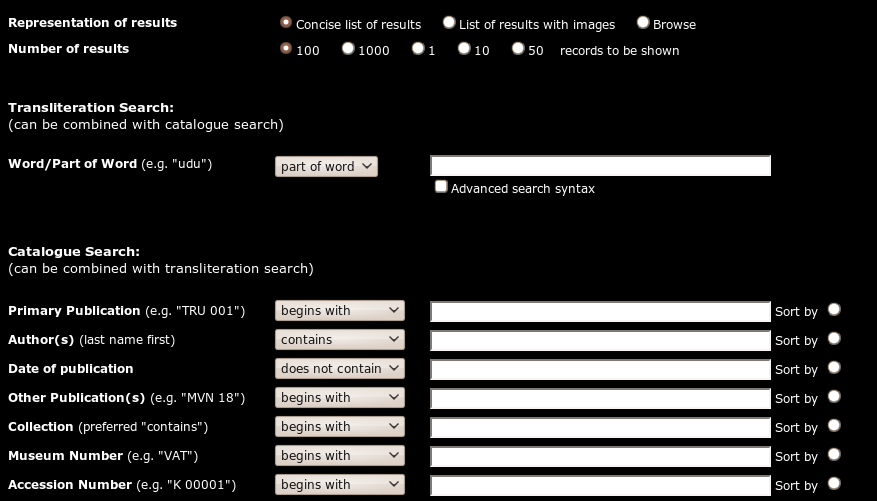
\includegraphics[width=300px]{../diagramy/cdli-search.png}
 % cdli-search.png: 877x501 pixel, 72dpi, 30.94x17.67 cm, bb=0 0 877 501
 \caption{Formularz wyszukiwania na CDLI}
 \label{fig:cdli-search}
\end{figure}

(http://cdli.ucla.edu) - największa znana nam baza tekstów sumeryjskich (ok. 225 tys. tekstów), 
wyszukiwanie po praktycznie wszystkich możliwych parametrach, choć trochę mało wygodne. Dla każdej metadanej jest pole tekstowe z możliwymi opcjami wyszukiwania: ``begins with``, ``contains'', ''does not contain''. Dla treści jest pole tekstowe z opcjami ``word``, ``part of word`` oraz checkbox ''advanced search syntax''. Brakuje wyjaśnienia jak 
używać ``Advanced search syntax''. Brakuje możliwości tworzenia złożonych zapytań.

\section{The Electronic Text Corpus of Sumerian Literature} 
\begin{figure}[h]
 \centering
 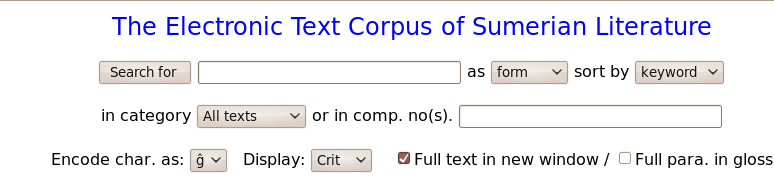
\includegraphics[width=300px]{../diagramy/etcsl-search.png}
 % etcsl-search.png: 774x182 pixel, 72dpi, 27.31x6.42 cm, bb=0 0 774 182
 \caption{Formularz wyszukiwania na etcsl}
 \label{fig:etcsl-search}
\end{figure}

(http://etcsl.orinst.ox.ac.uk/) - baza znacznie mniejsza, zawiera 
głównie teksty literackie. Wyszukiwanie mało rozbudowane.

